% Options for packages loaded elsewhere
\PassOptionsToPackage{unicode}{hyperref}
\PassOptionsToPackage{hyphens}{url}
\PassOptionsToPackage{dvipsnames,svgnames,x11names}{xcolor}
%
\documentclass[
  10pt,
]{krantz}
\usepackage{amsmath,amssymb}
\usepackage{iftex}
\ifPDFTeX
  \usepackage[T1]{fontenc}
  \usepackage[utf8]{inputenc}
  \usepackage{textcomp} % provide euro and other symbols
\else % if luatex or xetex
  \usepackage{unicode-math} % this also loads fontspec
  \defaultfontfeatures{Scale=MatchLowercase}
  \defaultfontfeatures[\rmfamily]{Ligatures=TeX,Scale=1}
\fi
\usepackage{lmodern}
\ifPDFTeX\else
  % xetex/luatex font selection
\fi
% Use upquote if available, for straight quotes in verbatim environments
\IfFileExists{upquote.sty}{\usepackage{upquote}}{}
\IfFileExists{microtype.sty}{% use microtype if available
  \usepackage[]{microtype}
  \UseMicrotypeSet[protrusion]{basicmath} % disable protrusion for tt fonts
}{}
\makeatletter
\@ifundefined{KOMAClassName}{% if non-KOMA class
  \IfFileExists{parskip.sty}{%
    \usepackage{parskip}
  }{% else
    \setlength{\parindent}{0pt}
    \setlength{\parskip}{6pt plus 2pt minus 1pt}}
}{% if KOMA class
  \KOMAoptions{parskip=half}}
\makeatother
\usepackage{xcolor}
\usepackage{color}
\usepackage{fancyvrb}
\newcommand{\VerbBar}{|}
\newcommand{\VERB}{\Verb[commandchars=\\\{\}]}
\DefineVerbatimEnvironment{Highlighting}{Verbatim}{commandchars=\\\{\}}
% Add ',fontsize=\small' for more characters per line
\usepackage{framed}
\definecolor{shadecolor}{RGB}{248,248,248}
\newenvironment{Shaded}{\begin{snugshade}}{\end{snugshade}}
\newcommand{\AlertTok}[1]{\textcolor[rgb]{0.94,0.16,0.16}{#1}}
\newcommand{\AnnotationTok}[1]{\textcolor[rgb]{0.56,0.35,0.01}{\textbf{\textit{#1}}}}
\newcommand{\AttributeTok}[1]{\textcolor[rgb]{0.13,0.29,0.53}{#1}}
\newcommand{\BaseNTok}[1]{\textcolor[rgb]{0.00,0.00,0.81}{#1}}
\newcommand{\BuiltInTok}[1]{#1}
\newcommand{\CharTok}[1]{\textcolor[rgb]{0.31,0.60,0.02}{#1}}
\newcommand{\CommentTok}[1]{\textcolor[rgb]{0.56,0.35,0.01}{\textit{#1}}}
\newcommand{\CommentVarTok}[1]{\textcolor[rgb]{0.56,0.35,0.01}{\textbf{\textit{#1}}}}
\newcommand{\ConstantTok}[1]{\textcolor[rgb]{0.56,0.35,0.01}{#1}}
\newcommand{\ControlFlowTok}[1]{\textcolor[rgb]{0.13,0.29,0.53}{\textbf{#1}}}
\newcommand{\DataTypeTok}[1]{\textcolor[rgb]{0.13,0.29,0.53}{#1}}
\newcommand{\DecValTok}[1]{\textcolor[rgb]{0.00,0.00,0.81}{#1}}
\newcommand{\DocumentationTok}[1]{\textcolor[rgb]{0.56,0.35,0.01}{\textbf{\textit{#1}}}}
\newcommand{\ErrorTok}[1]{\textcolor[rgb]{0.64,0.00,0.00}{\textbf{#1}}}
\newcommand{\ExtensionTok}[1]{#1}
\newcommand{\FloatTok}[1]{\textcolor[rgb]{0.00,0.00,0.81}{#1}}
\newcommand{\FunctionTok}[1]{\textcolor[rgb]{0.13,0.29,0.53}{\textbf{#1}}}
\newcommand{\ImportTok}[1]{#1}
\newcommand{\InformationTok}[1]{\textcolor[rgb]{0.56,0.35,0.01}{\textbf{\textit{#1}}}}
\newcommand{\KeywordTok}[1]{\textcolor[rgb]{0.13,0.29,0.53}{\textbf{#1}}}
\newcommand{\NormalTok}[1]{#1}
\newcommand{\OperatorTok}[1]{\textcolor[rgb]{0.81,0.36,0.00}{\textbf{#1}}}
\newcommand{\OtherTok}[1]{\textcolor[rgb]{0.56,0.35,0.01}{#1}}
\newcommand{\PreprocessorTok}[1]{\textcolor[rgb]{0.56,0.35,0.01}{\textit{#1}}}
\newcommand{\RegionMarkerTok}[1]{#1}
\newcommand{\SpecialCharTok}[1]{\textcolor[rgb]{0.81,0.36,0.00}{\textbf{#1}}}
\newcommand{\SpecialStringTok}[1]{\textcolor[rgb]{0.31,0.60,0.02}{#1}}
\newcommand{\StringTok}[1]{\textcolor[rgb]{0.31,0.60,0.02}{#1}}
\newcommand{\VariableTok}[1]{\textcolor[rgb]{0.00,0.00,0.00}{#1}}
\newcommand{\VerbatimStringTok}[1]{\textcolor[rgb]{0.31,0.60,0.02}{#1}}
\newcommand{\WarningTok}[1]{\textcolor[rgb]{0.56,0.35,0.01}{\textbf{\textit{#1}}}}
\usepackage{longtable,booktabs,array}
\usepackage{calc} % for calculating minipage widths
% Correct order of tables after \paragraph or \subparagraph
\usepackage{etoolbox}
\makeatletter
\patchcmd\longtable{\par}{\if@noskipsec\mbox{}\fi\par}{}{}
\makeatother
% Allow footnotes in longtable head/foot
\IfFileExists{footnotehyper.sty}{\usepackage{footnotehyper}}{\usepackage{footnote}}
\makesavenoteenv{longtable}
\usepackage{graphicx}
\makeatletter
\newsavebox\pandoc@box
\newcommand*\pandocbounded[1]{% scales image to fit in text height/width
  \sbox\pandoc@box{#1}%
  \Gscale@div\@tempa{\textheight}{\dimexpr\ht\pandoc@box+\dp\pandoc@box\relax}%
  \Gscale@div\@tempb{\linewidth}{\wd\pandoc@box}%
  \ifdim\@tempb\p@<\@tempa\p@\let\@tempa\@tempb\fi% select the smaller of both
  \ifdim\@tempa\p@<\p@\scalebox{\@tempa}{\usebox\pandoc@box}%
  \else\usebox{\pandoc@box}%
  \fi%
}
% Set default figure placement to htbp
\def\fps@figure{htbp}
\makeatother
\setlength{\emergencystretch}{3em} % prevent overfull lines
\providecommand{\tightlist}{%
  \setlength{\itemsep}{0pt}\setlength{\parskip}{0pt}}
\setcounter{secnumdepth}{5}
\usepackage{booktabs}
\usepackage{longtable}
\usepackage[bf,singlelinecheck=off]{caption}
\usepackage{hyperref}
\usepackage{Alegreya}
\usepackage[scale=.7]{sourcecodepro}

\usepackage{framed,color}
\definecolor{shadecolor}{RGB}{248,248,248}

\renewcommand{\textfraction}{0.05}
\renewcommand{\topfraction}{0.8}
\renewcommand{\bottomfraction}{0.8}
\renewcommand{\floatpagefraction}{0.75}

\renewenvironment{quote}{\begin{VF}}{\end{VF}}
\let\oldhref\href
\renewcommand{\href}[2]{#2\footnote{\url{#1}}}

\ifxetex
  \usepackage{letltxmacro}
  \setlength{\XeTeXLinkMargin}{1pt}
  \LetLtxMacro\SavedIncludeGraphics\includegraphics
  \def\includegraphics#1#{% #1 catches optional stuff (star/opt. arg.)
    \IncludeGraphicsAux{#1}%
  }%
  \newcommand*{\IncludeGraphicsAux}[2]{%
    \XeTeXLinkBox{%
      \SavedIncludeGraphics#1{#2}%
    }%
  }%
\fi

\makeatletter
\newenvironment{kframe}{%
\medskip{}
\setlength{\fboxsep}{.8em}
 \def\at@end@of@kframe{}%
 \ifinner\ifhmode%
  \def\at@end@of@kframe{\end{minipage}}%
  \begin{minipage}{\columnwidth}%
 \fi\fi%
 \def\FrameCommand##1{\hskip\@totalleftmargin \hskip-\fboxsep
 \colorbox{shadecolor}{##1}\hskip-\fboxsep
     % There is no \\@totalrightmargin, so:
     \hskip-\linewidth \hskip-\@totalleftmargin \hskip\columnwidth}%
 \MakeFramed {\advance\hsize-\width
   \@totalleftmargin\z@ \linewidth\hsize
   \@setminipage}}%
 {\par\unskip\endMakeFramed%
 \at@end@of@kframe}
\makeatother

\makeatletter
\@ifundefined{Shaded}{
}{\renewenvironment{Shaded}{\begin{kframe}}{\end{kframe}}}
\makeatother

\newenvironment{rmdblock}[1]
  {
  \begin{itemize}
  \renewcommand{\labelitemi}{
    \raisebox{-.7\height}[0pt][0pt]{
      {\setkeys{Gin}{width=3em,keepaspectratio}\includegraphics{images/#1}}
    }
  }
  \setlength{\fboxsep}{1em}
  \begin{kframe}
  \item
  }
  {
  \end{kframe}
  \end{itemize}
  }
\newenvironment{rmdnote}
  {\begin{rmdblock}{note}}
  {\end{rmdblock}}
\newenvironment{rmdcaution}
  {\begin{rmdblock}{caution}}
  {\end{rmdblock}}
\newenvironment{rmdimportant}
  {\begin{rmdblock}{important}}
  {\end{rmdblock}}
\newenvironment{rmdtip}
  {\begin{rmdblock}{tip}}
  {\end{rmdblock}}
\newenvironment{rmdwarning}
  {\begin{rmdblock}{warning}}
  {\end{rmdblock}}

\usepackage{makeidx}
\makeindex

\urlstyle{tt}

\usepackage{amsthm}
\makeatletter
\def\thm@space@setup{%
  \thm@preskip=8pt plus 2pt minus 4pt
  \thm@postskip=\thm@preskip
}
\makeatother

\frontmatter
\usepackage[]{natbib}
\bibliographystyle{apalike}
\usepackage{bookmark}
\IfFileExists{xurl.sty}{\usepackage{xurl}}{} % add URL line breaks if available
\urlstyle{same}
\hypersetup{
  pdftitle={Predictive Analytics},
  pdfauthor={Jeff Maxey},
  colorlinks=true,
  linkcolor={Maroon},
  filecolor={Maroon},
  citecolor={Blue},
  urlcolor={Blue},
  pdfcreator={LaTeX via pandoc}}

\title{Predictive Analytics}
\author{Jeff Maxey}
\date{2025-03-16}

\begin{document}
\maketitle

%\cleardoublepage\newpage\thispagestyle{empty}\null
%\cleardoublepage\newpage\thispagestyle{empty}\null
%\cleardoublepage\newpage
\thispagestyle{empty}
\begin{center}
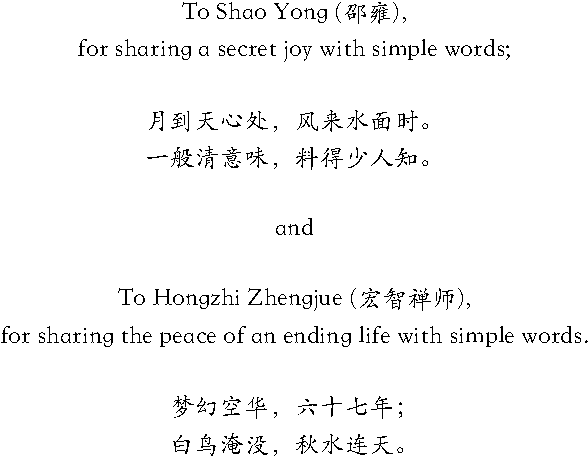
\includegraphics{images/dedication.pdf}
\end{center}

\setlength{\abovedisplayskip}{-5pt}
\setlength{\abovedisplayshortskip}{-5pt}

{
\hypersetup{linkcolor=}
\setcounter{tocdepth}{2}
\tableofcontents
}
\listoffigures
\listoftables
\chapter*{Preface}\label{preface}


This short book introduces an R package, \textbf{bookdown}, to change your workflow of writing books. It should be technically easy to write a book, visually pleasant to view the book, fun to interact with the book, convenient to navigate through the book, straightforward for readers to contribute or leave feedback to the book author(s), and more importantly, authors should not always be distracted by typesetting details.

The \textbf{bookdown} package is built on top of R Markdown (\url{http://rmarkdown.rstudio.com}), and inherits the simplicity of the Markdown syntax (you can learn the basics in five minutes; see Section \ref{markdown-syntax}), as well as the possibility of multiple types of output formats (PDF/HTML/Word/\ldots). It has also added features like multi-page HTML output, numbering and cross-referencing figures/tables/sections/equations, inserting parts/appendices, and imported the GitBook\index{GitBook} style (\url{https://www.gitbook.com}) to create elegant and appealing HTML book pages. This book itself is an example of how you can produce a book from a series of R Markdown documents, and both the printed version and the online version can look professional. You can find more examples at \url{https://bookdown.org}.

Despite the package name containing the word ``book'', \textbf{bookdown} is not only for books. The ``book'' can be anything that consists of multiple R Markdown documents meant to be read in a linear sequence, such as course handouts, study notes, a software manual, a thesis, or even a diary. In fact, many \textbf{bookdown} features apply to single R Markdown documents as well (see Section \ref{a-single-document}).

\pandocbounded{
\includegraphics[keepaspectratio]{images/by-nc-sa.png}}\\
The online version of this book is licensed under the \href{http://creativecommons.org/licenses/by-nc-sa/4.0/}{Creative Commons Attribution-NonCommercial-ShareAlike 4.0 International License}. You can purchase a hardcopy from \href{https://www.crcpress.com/product/isbn/9781138700109}{Chapman \& Hall} or Amazon.

\section*{Why read this book}\label{why-read-this-book}


Can we write a book in one source format, and generate the output to multiple formats? Traditionally books are often written with LaTeX or Microsoft Word. Either of these tools will make writing books a one-way trip and you cannot turn back: if you choose LaTeX, you typically end up only with a PDF document; if you work with Word, you are likely to have to stay in Word forever, and may also miss the many useful features and beautiful PDF output from LaTeX.

Can we focus on writing the content without worrying too much about typesetting? There seems a natural contradiction between content and appearance, and we always have to balance our time spent on these two aspects. No one can have a cake and eat it too, but it does not mean we cannot have a half and eat a half. We want our book to look reasonably pretty, and we also want to focus on the content. One possibility is to give up PDF temporarily, and what you may have in return is a pretty preview of your book as HTML web pages\index{HTML}. LaTeX\index{LaTeX} is an excellent typesetting tool, but you can be easily buried in the numerous LaTeX commands and typesetting details while you are working on the book. It is just so hard to refrain from previewing the book in PDF, and unfortunately also so common to find certain words exceed the page margin, certain figures float to a random page, five or six stray words at the very end of a chapter proudly take up a whole new page, and so on. If the book is to be printed, we will have to deal with these issues eventually, but it is not worth being distracted over and over again while you are writing the content of the book. The fact that the Markdown syntax is simpler and has fewer features than LaTeX also helps you focus on the content. Do you really have to define a new command like \texttt{\textbackslash{}myprecious\{\}} that applies \texttt{\textbackslash{}textbf\{\textbackslash{}textit\{\textbackslash{}textsf\{\}\}\}} to your text? Does the letter ``R'' have to be enclosed in \texttt{\textbackslash{}proglang\{\}} when readers can easily figure out it stands for the R language? It does not make much difference whether everything, or nothing, needs the reader's attention.

Can readers interact with examples in our book as they read it? The answer is certainly no if the book is printed on paper, but it is possible if your book has an HTML version that contains live examples, such as Shiny applications (\url{https://shiny.rstudio.com}) or HTML widgets (\url{https://htmlwidgets.org}). For example, readers may immediately know what happens if they change certain parameters of a statistical model.

Can we get feedback and even contributions from readers as we develop the book? Traditionally the editor will find a small number of anonymous reviewers to review your book. Reviewers are often helpful, but you may still miss the wisdom of more representative readers. It is too late after the first edition is printed, and readers may need to wait for a few years before the second edition is ready. There are some web platforms that make it easy for people to provide feedback and contribute to your projects. GitHub (\url{https://github.com}) is one prominent example. If anyone finds a typo in your book, he/she can simply correct it online and submit the change back to you for your approval. It is a matter of clicking a button to merge the change, with no questions asked or emails back and forth. To be able to use these platforms, you need to learn the basics of version control tools like GIT, and your book source files should be in plain text.

The combination of R (\url{https://www.r-project.org}), Markdown, and Pandoc (\url{http://pandoc.org}) makes it possible to go from one simple source format (R Markdown) to multiple possible output formats (PDF, HTML, EPUB, and Word, etc.). The \textbf{bookdown} package is based on R Markdown, and provides output formats for books and long-form articles, including the GitBook format, which is a multi-page HTML output format with a useful and beautiful user interface. It is much easier to typeset in HTML than LaTeX, so you can always preview your book in HTML, and work on PDF after the content is mostly done. Live examples can be easily embedded in HTML, which can make the book more attractive and useful. R Markdown is a plain-text format, so you can also enjoy the benefits of version control, such as collaborating on GitHub. We have also tried hard to port some important features from LaTeX to HTML and other output formats, such as figure/table numbering and cross-references.

In short, you just prepare a few R Markdown book chapters, and \textbf{bookdown} can help you turn them into a beautiful book.

\section*{Structure of the book}\label{structure-of-the-book}


Chapters \ref{introduction} and \ref{components} introduce the basic usage and syntax, which should be sufficient to get most readers started in writing a book. Chapters \ref{output-formats} and \ref{customization} are for those who want to fine-tune the appearance of their books. They may look very technical if you are not familiar with HTML/CSS and LaTeX. You do not need to read these two chapters very carefully for the first time. You can learn what can be possibly changed, and come back later to know how. For Chapter \ref{editing}, the technical details are not important unless you do not use the RStudio IDE (Section \ref{rstudio-ide}). Similarly, you may feel overwhelmed by the commands presented in Chapter \ref{publishing} to publish your book, but again, we have tried to make it easy to publish your book online via the RStudio IDE. The custom commands and functions are only for those who choose not to use RStudio's service or want to understand the technical details.

To sum it up, this book is a comprehensive reference of the \textbf{bookdown} package. You can follow the \href{https://en.wikipedia.org/wiki/Pareto_principle}{80/20 rule} when reading it. Some sections are there for the sake of completeness, and not all sections are equally useful to the particular book(s) that you intend to write.

\section*{Software information and conventions}\label{software-information-and-conventions}


This book is primarily about the R package \textbf{bookdown}, so you need to at least install R and the \textbf{bookdown} package. However, your book does not have to be related to the R language at all. It can use other computing languages (C++, SQL, Python, and so on; see Appendix \ref{software-usage}), and it can even be totally irrelevant to computing (e.g., you can write a novel, or a collection of poems). The software tools required to build a book are introduced in Appendix \ref{software-tools}.

The R session information when compiling this book is shown below:

\begin{Shaded}
\begin{Highlighting}[]
\FunctionTok{sessionInfo}\NormalTok{()}
\end{Highlighting}
\end{Shaded}

\begin{verbatim}
## R version 4.4.3 (2025-02-28 ucrt)
## Platform: x86_64-w64-mingw32/x64
## Running under: Windows 11 x64 (build 26100)
## 
## Matrix products: default
## 
## 
## locale:
## [1] LC_COLLATE=English_United States.utf8 
## [2] LC_CTYPE=English_United States.utf8   
## [3] LC_MONETARY=English_United States.utf8
## [4] LC_NUMERIC=C                          
## [5] LC_TIME=English_United States.utf8    
## 
## time zone: America/Chicago
## tzcode source: internal
## 
## attached base packages:
## [1] stats     graphics  grDevices datasets  utils    
## [6] methods   base     
## 
## loaded via a namespace (and not attached):
## [1] bookdown_0.42     shiny_1.10.0     
## [3] miniUI_0.1.1.1    knitr_1.49       
## [5] htmltools_0.5.8.1 rmarkdown_2.29   
## [7] tools_4.4.3
\end{verbatim}

We do not add prompts (\texttt{\textgreater{}} and \texttt{+}) to R source code in this book, and we comment out the text output with two hashes \texttt{\#\#} by default, as you can see from the R session information above. This is for your convenience when you want to copy and run the code (the text output will be ignored since it is commented out). Package names are in bold text (e.g., \textbf{rmarkdown}), and inline code and filenames are formatted in a typewriter font (e.g., \texttt{knitr::knit(\textquotesingle{}foo.Rmd\textquotesingle{})}). Function names are followed by parentheses (e.g., \texttt{bookdown::render\_book()}). The double-colon operator \texttt{::} means accessing an object from a package.

\section*{Acknowledgments}\label{acknowledgments}


First I'd like to thank my employer, RStudio, for providing me the opportunity to work on this exciting project. I was hoping to work on it when I first saw the GitBook project in 2013, because I immediately realized it was a beautiful book style and there was a lot more power we could add to it, judging from my experience of writing the \textbf{knitr} book \citep{xie2015} and reading other books. R Markdown became mature after two years, and luckily, \textbf{bookdown} became my official job in late 2015. There are not many things in the world better than the fact that your job happens to be your hobby (or vice versa). I totally enjoyed messing around with JavaScript libraries, LaTeX packages, and endless regular expressions in R. Honestly I should also thank Stack Overflow (\url{https://stackoverflow.com}), and I believe you all know \href{http://bit.ly/2cWbiAp}{what I mean,} if you have ever written any program code.

This project is certainly not a single person's effort. Several colleagues at RStudio have helped me along the way. Hadley Wickham provided a huge amount of feedback during the development of \textbf{bookdown}, as he was working on his book \emph{R for Data Science} with Garrett Grolemund. JJ Allaire and Jonathan McPherson provided a lot of technical help directly to this package as well as support in the RStudio IDE. Jeff Allen, Chaita Chaudhari, and the RStudio Connect team have been maintaining the \url{https://bookdown.org} website. Robby Shaver designed a nice cover image for this book. Both Hadley Wickham and Mine Cetinkaya-Rundel reviewed the manuscript and gave me a lot of helpful comments. Tareef Kawaf tried his best to help me become a professional software engineer. It is such a blessing to work in this company with enthusiastic and smart people. I remember once I told Jonathan, ``hey I found a problem in caching HTML widgets dependencies and finally figured out a possible solution''. Jonathan grabbed his beer and said, ``I already solved it.'' ``Oh, nice, nice.''

I also received a lot of feedback from book authors outside RStudio, including Jan de Leeuw, Jenny Bryan, Dean Attali, Rafael Irizarry, Michael Love, Roger Peng, Andrew Clark, and so on. Some users also contributed code to the project and helped revise the book. Here is a list of all contributors: \url{https://github.com/rstudio/bookdown/graphs/contributors}. It feels good when you invent a tool and realize you are also the beneficiary of your own tool. As someone who loves the GitHub pull request model, I wished readers did not have to email me there was a typo or obvious mistake in my book, but could just fix it via a pull request. This was made possible in \textbf{bookdown}. You can see how many pull requests on typos I have merged: \url{https://github.com/rstudio/bookdown/pulls}. It is nice to have so many outsourced careful human spell checkers. It is not that I do not know how to use a real spell checker, but I do not want to do this before the book is finished, and the evil Yihui also wants to leave a few simple tasks to the readers to engage them in improving the book.

Callum Webb kindly designed a nice hexbin sticker for \textbf{bookdown}.

The \textbf{bookdown} package is not possible without a few open-source software packages. In particular, Pandoc, GitBook, jQuery, and the dependent R packages, not to mention R itself. I thank the developers of these packages.

I moved to Omaha, Nebraska, in 2015, and enjoyed one year at Steeplechase Apartments, where I lived comfortably while developing the \textbf{bookdown} package, thanks to the extremely friendly and helpful staff. Then I met a professional and smart realtor, Kevin Schaben, who found a fabulous home for us in an amazingly short period of time, and I finished this book in our new home.

John Kimmel, the editor from Chapman \& Hall/CRC, helped me publish my first book. It is my pleasure to work with him again. He generously agreed to let me keep the online version of this book for free, so I can continue to update it after it is printed and published (i.e., you do not have to wait for years for the second edition to correct mistakes and introduce new features). I wish I could be as open-minded as he is when I'm his age. Rebecca Condit and Suzanne Lassandro proofread the manuscript, and their suggestions were professional and helpful. Shashi Kumar solved some of my technical issues with the publisher's LaTeX class (\texttt{krantz.cls}) when I was trying to integrate it with \textbf{bookdown}. I also appreciate the very helpful comments from the reviewers Jan de Leeuw, Karl Broman, Brooke Anderson, Michael Grayling, Daniel Kaplan, and Max Kuhn.

Lastly I want to thank my family, in particular, my wife and son, for their support. The one-year-old has discovered that my monitor will light up when he touches my keyboard, so occasionally he just creeps into my office and presses randomly on the keyboard when I'm away. I'm not sure if this counts as his contribution to the book\ldots{} @)!\%)\&@*

\begin{flushright}
Yihui Xie\\
Elkhorn, Nebraska
\end{flushright}

\part{Introduction to Predictive Analytics}\label{part-introduction-to-predictive-analytics}

\chapter{Overview of Predictive Analytics}\label{overview-of-predictive-analytics}

\section*{Introduction}\label{introduction}


This foundational chapter streamlines the material scattered in different parts
of the PA e-learning modules and provides a broad and coherent introduction to
predictive analytics.

Setting the scene for pretty much everything that comes later, it walks you
through the main steps in building a predictive model and presents the
fundamental concepts in predictive analytics that you will see repeatedly in the
rest of this manual.

These concepts are universally applicable in the sense that they apply to
essentially all types of predictive model, and will be illustrated in the
context of specific types of model (GLMs and decision trees, in particular) in
later chapters.

\section{Basic Terminology}\label{basic-terminology}

\textbf{Predictive Analytics in a nutshell.} Three main categories of predictive
analytics problems:

\begin{itemize}
\item
  \textbf{\emph{Descriptive:}} Focuses on what happened in the past and aims to
  ``describe'' or explain the observed patterns by identifying the relationships
  between different variables in the data.

  \textbf{Example.} If you saw an increase in the lapse rate among the
  policyholders of a certain line of business, what kind of policyholders had
  the highest tendency to lapse? What are their key characteristics? This is a
  question addressed by descriptive analytics.
\item
  \textbf{\emph{Predictive:}} Focuses on what will happen in the \emph{future} and is
  concerned with making accurate ``predictions''.

  \textbf{Example:} For a prospective policyholder with certain characteristics,
  what is their predicted probability of lapse? The ability to make such a
  prediction will be useful for identifying future policyholders who will have
  a lower probability of lapse and contribute to the profitability of an
  insurer.
\item
  \textbf{\emph{Prescriptive:}} Uses a combination of optimization and simulation to
  quantify the impact of different ``prescribed'' actions in different
  scenarios.

  \textbf{Example:} If we reduce the premium by a certain amount, how will this
  affect the lapse rate? More generally, what is the best course of action to
  reduce the lapse rate? Prescriptive analytics may give us some useful
  insight.
\end{itemize}

All predictive problems have something in common. There is always an output (or
outcome) of interest, which can be numeric (salary, premium) or categorical
(positive/negative, email/spam), and we have at our disposal a collection of
input variables that may offer potentially useful information for predicting or
understanding the output.

This ``input-output'' setting, depicted below, is characteristic of predictive
analytics in general, and our job is to develop a model teasing the (possibly
complex, overlapping) contributions of the inputs to the output.

\[
\underset{\underset{Output}{\text{Target Variable}}}{Y} \overset{\text{Predict}}{\underset{\text{}}{\dashleftarrow}}\underset{\underset{Inputs}{\text{Predictors}}}{X = (X_1,...,Xp)}
\]

\textbf{Classification of Variables.} Predictive analytics requires data, often with
a large number of observations and variables. In Exam PA, we will be mostly
dealing with datasets that can be displayed in the following
observation-by-variable rectangular array format (such data is called
\textbf{\emph{structured data}} and is stored in \texttt{R} in a data frame).

\begin{longtable}[]{@{}
  >{\centering\arraybackslash}p{(\linewidth - 10\tabcolsep) * \real{0.2436}}
  >{\centering\arraybackslash}p{(\linewidth - 10\tabcolsep) * \real{0.1795}}
  >{\centering\arraybackslash}p{(\linewidth - 10\tabcolsep) * \real{0.2308}}
  >{\centering\arraybackslash}p{(\linewidth - 10\tabcolsep) * \real{0.1282}}
  >{\centering\arraybackslash}p{(\linewidth - 10\tabcolsep) * \real{0.0897}}
  >{\centering\arraybackslash}p{(\linewidth - 10\tabcolsep) * \real{0.1282}}@{}}
\caption{Structured Data Format}\tabularnewline
\toprule\noalign{}
\begin{minipage}[b]{\linewidth}\centering
\textbf{\emph{Observation}}
\end{minipage} & \begin{minipage}[b]{\linewidth}\centering
\textbf{\emph{Target}}
\end{minipage} & \begin{minipage}[b]{\linewidth}\centering
\textbf{\emph{Predictors}}
\end{minipage} & \begin{minipage}[b]{\linewidth}\centering
\end{minipage} & \begin{minipage}[b]{\linewidth}\centering
\end{minipage} & \begin{minipage}[b]{\linewidth}\centering
\end{minipage} \\
\midrule\noalign{}
\endfirsthead
\toprule\noalign{}
\begin{minipage}[b]{\linewidth}\centering
\textbf{\emph{Observation}}
\end{minipage} & \begin{minipage}[b]{\linewidth}\centering
\textbf{\emph{Target}}
\end{minipage} & \begin{minipage}[b]{\linewidth}\centering
\textbf{\emph{Predictors}}
\end{minipage} & \begin{minipage}[b]{\linewidth}\centering
\end{minipage} & \begin{minipage}[b]{\linewidth}\centering
\end{minipage} & \begin{minipage}[b]{\linewidth}\centering
\end{minipage} \\
\midrule\noalign{}
\endhead
\bottomrule\noalign{}
\endlastfoot
& \(Y\) & \(X_1\) & \(X_2\) & \(...\) & \(X_p\) \\
\(1\) & \(Y_1\) & \(X_{11}\) & \(X_{12}\) & \(...\) & \(X_{1p}\) \\
\(2\) & \(Y_2\) & \(X_{21}\) & \(X_{22}\) & \(...\) & \(X_{2p}\) \\
\(...\) & \(...\) & \(...\) & \(...\) & \(...\) & \(...\) \\
\(n\) & \(Y_n\) & \(X_{n1}\) & \(X_{n2}\) & \(...\) & \(X_{np}\) \\
\end{longtable}

\section{The Model Building Process}\label{the-model-building-process}

\section{Bias-Variance Trade-off}\label{bias-variance-trade-off}

\section{Feature Generation and Selection}\label{feature-generation-and-selection}

\section{Conceptual Review Questions for Chapter 1}\label{conceptual-review-questions-for-chapter-1}

\chapter{Data Exploration and Visualization}\label{data-exploration-and-visualization}

\section{Univariate Data Exploration}\label{univariate-data-exploration}

\section{Bivariate Data Exploration}\label{bivariate-data-exploration}

\section{Conceptual Review Questions for Chapter 2}\label{conceptual-review-questions-for-chapter-2}

  \bibliography{book.bib,packages.bib}

\printindex

\end{document}
